\section{О металлическом водороде}

Что такое металл? Кто-то наверное думает, что металлы это вещества из нижнего треугольника периодической системы элементов Менделеева. Это правда, но при условии, что температура в районе 273 К, давление в районе 1 атм, и мы исключили все полупроводники. Металл это прежде всего хороший проводник. Но что такое хороший проводник? С точки зрения классической теории это вещество с большой проводимостью. Есть чёткие границы, но они, как это ясно, размываются при изменении температуры и давления. С точки зрения квантовой теории это вещества, в которых есть зона проводимости. Мне трудно охарактеризовать её словами, поэтому вот рисунок:
\begin{center}
	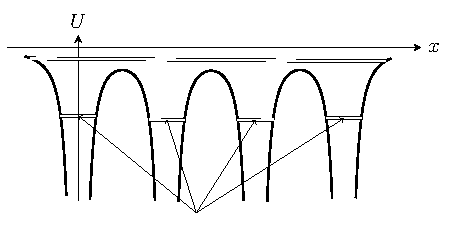
\includegraphics[width = 0.6\textwidth]{images/tikz/for_H_metall}
\end{center}